\section{标准输出和变量}

\subsection{printf函数}

打开visual studio,在“源文件”上右键,点击“添加”->“新建项”,创建一个叫main.c的文件,在其中输入

\begin{lstlisting}[language=C]
    #include <stdio.h>
    
    int main() {
        printf("Hello World!");

        return 0;
    }
\end{lstlisting}

点击“本地Windows调试器”,将会出现类似于这样的界面

\begin{figure}[H]
    \centering
    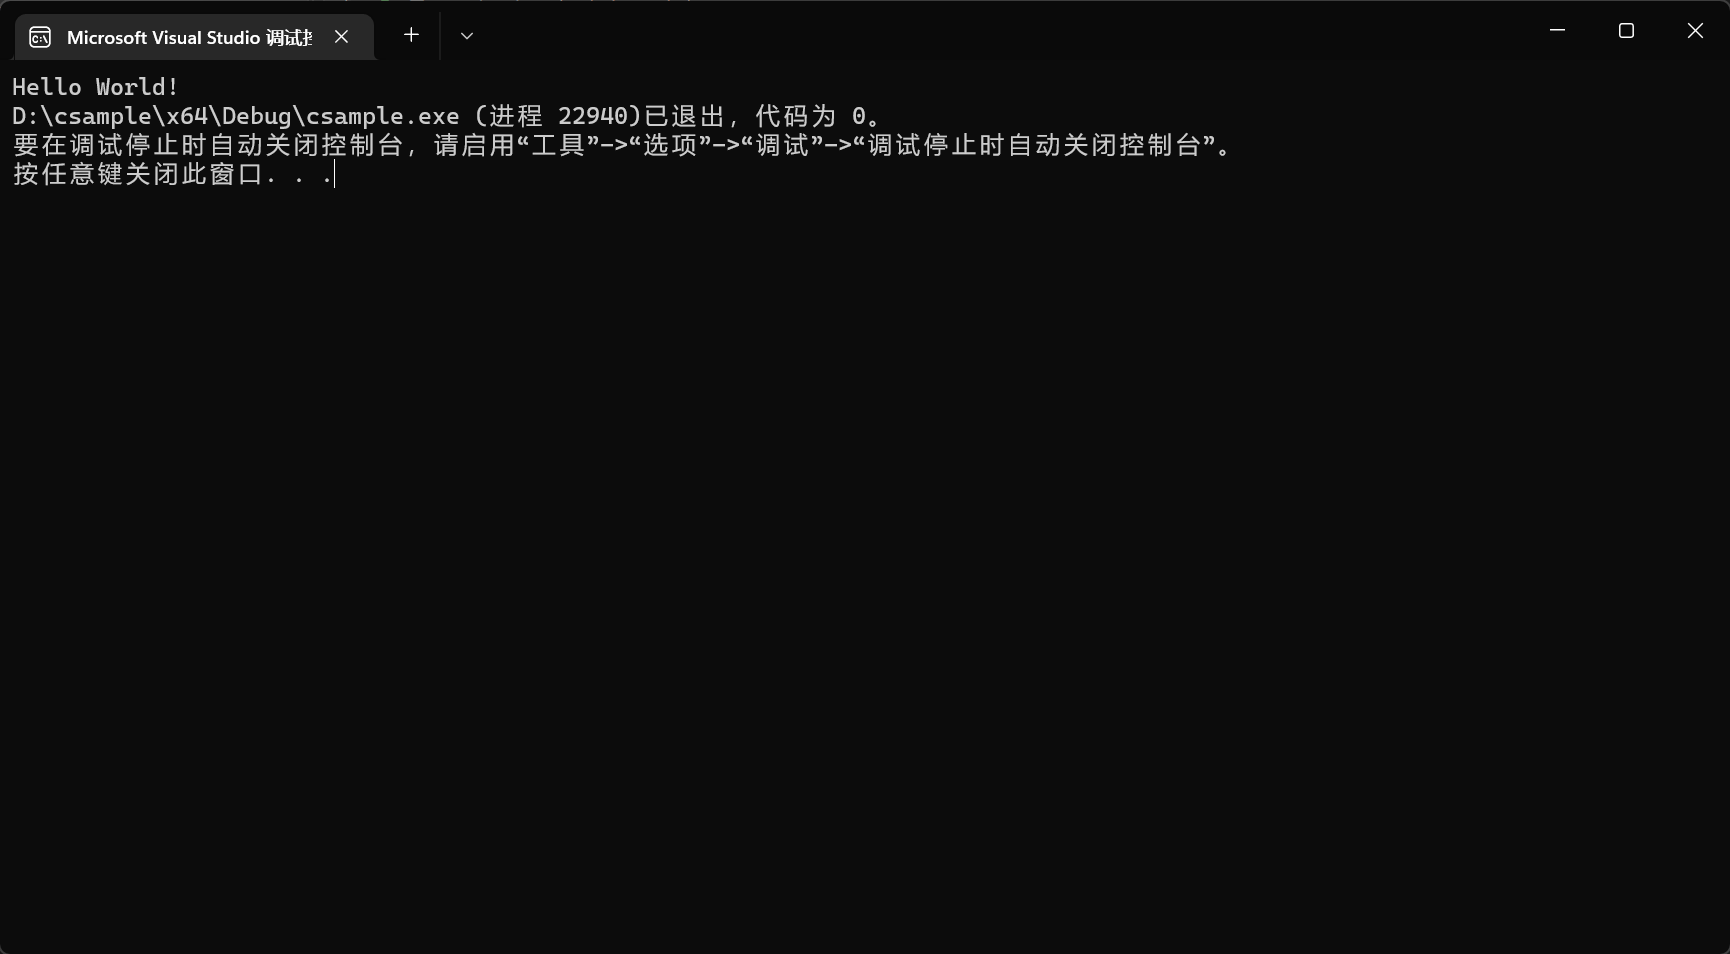
\includegraphics[width=0.8\textwidth, height=0.4\textheight]{images/1HelloWorld结果.png}
\end{figure}

恭喜你写出了你的第一段代码。计算机领域有一个传统:刚入门编程的人的第一段代码一定要是Hello World,这是我们对无垠的计算机世界打的招呼。这个黑乎乎的界面叫做终端(这里不做关于终端、shell等的详细区分),我们以后会常常和它打交道。

我们发现,我们写在printf的引号内的内容会被打印出来(顾名思义,printf就是print function嘛\footnote{事实并非如此,实际上此处的f指代format}),因此我们可以多写几个printf(不要忘了每行最后的英文分号),如

\begin{lstlisting}[language=C]
    #include <stdio.h>
    
    int main() {
        printf("Hello World!");
        printf("Potato");

        return 0;
    }
\end{lstlisting}

运行代码,我们观察到Hello World和Potato输出在了同一行。我们想要的是这二者各自占一行,那就需要在Hello World!后加一个换行符,也即$\backslash$n,代码就变成了

\begin{lstlisting}[language=C]
    #include <stdio.h>
    
    int main() {
        printf("Hello World!\n");
        printf("Potato\n");

        return 0;
    }
\end{lstlisting}

这次的结果就是我们想要的了。为什么Potato也要加换行符?这是因为也许我们在其后还会添加新的printf,要是到时候忘了给Potato加换行符,不就没有实现我们想要的效果吗?为了避免以后出现不必要的问题,我们推荐每个printf后都加换行符。

由上面的代码,我们总结出了这些要点:首先,我们要想输出信息,就要将其写在printf的引号内;其次,要想换行,就需要在输出的文本最后加一个换行符$\backslash$n;另外我们还注意到,我们先输出了Hello World,再输出了Potato,也就是说,程序是按照从上到下的顺序执行的。

这是很重要的结论,所以我们使用printf输出一遍加强印象吧。于是我们写下了:

\begin{lstlisting}[language=C]
    printf("首先,我们要想输出信息,就要将其写在printf的引号内;其次,要想换行,就需要在输出的文本最后加一个换行符\n;\n");
\end{lstlisting}

我们注意到有个问题,就是第一个换行符是我们想要按照文本形式输出的,但是如果按照上面的写法,它会被用于换行而不是直接输出。为了解决这个问题,我们把代码改成这样即可:

\begin{lstlisting}[language=C]
    printf("首先,我们要想输出信息,就要将其写在printf的引号内;其次,要想换行,就需要在输出的文本最后加一个换行符\\n;\n");
\end{lstlisting}

运行结果是:

\begin{figure}[H]
    \centering
    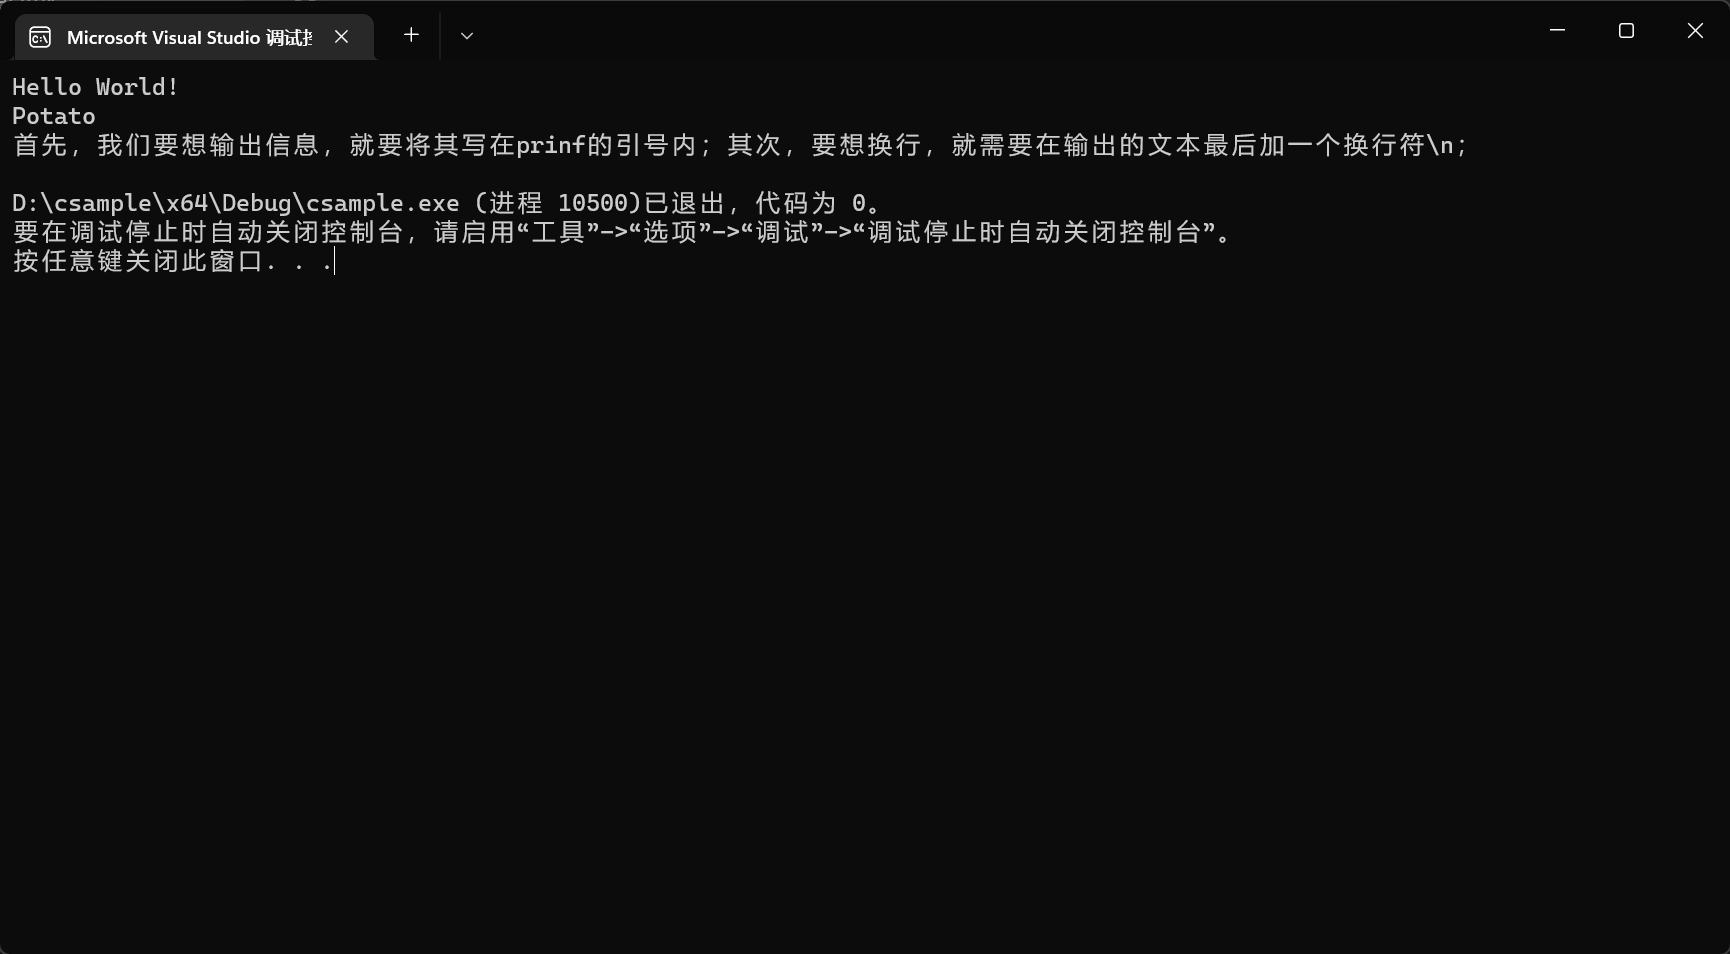
\includegraphics[width=0.8\textwidth, height=0.4\textheight]{images/1换行符输出.png}
\end{figure}

为什么会这样呢?实际上,我们输入的$\backslash$n和$\backslash{}\backslash$都叫做转义符号,用来实现一些特殊的输出效果。它的语法就是反斜杠($\backslash$)加一个字母。我们最常用的转义符号就是换行符$\backslash$n,实际上还有$\backslash$t、$\backslash$a等等。因为反斜杠会和下一个字母结合变成转义符号,所以要想输出反斜杠,就需要按照上面的例子那样使用两个反斜杠,这个转义符号的结果就是输出一个反斜杠。

\subsection{变量}

变量顾名思义,就是可以变的量。一个变量肯定要有名字,然后要有一个值。这就像是我们的考试成绩,有一个叫做“数学成绩”的变量,这次可以是120,下次可以是130。在c语言中,我们这样声明变量:$type\quad{}name$,啥意思呢,比如我们要声明数学成绩(math\_grade),那么就可以这样写

\begin{lstlisting}[language=C]
    int math_grade; 
\end{lstlisting}

这里的int是整数的意思,还有其它类型(如小数)我们之后会讲到。所以这行代码的意思就是,我们声明了一个叫做math\_grade的变量,它是一个整数。接下来就要给它赋值了,在大部分计算机语言中,赋值号都是=,比如数学成绩是120,那么就可以写

\begin{lstlisting}[language=C]
    math_grade = 120;
\end{lstlisting}

这段代码的意思就是给math\_grade赋予120这个值。也即,我们将赋值号右边的值给了左边的变量。我们强调是将右边的值赋给左边,说明了这不是数学中的等号,它不意味着左右两边相等,也不能交换左右两边的位置。

现在我们的main.c应该是这样的

\begin{lstlisting}[language=C]
    #include <stdio.h>

    int main() {
        int math_grade;
        math_grade = 120;

        return 0;
    }
\end{lstlisting}

第四行是声明变量,第五行是给变量赋值。如果我们在声明变量时就知道它要赋什么值,那么就可以把声明和赋值写在一起

\begin{lstlisting}[language=C]
    int math_grade = 120;
\end{lstlisting}

如果要同时声明多个类型一样的变量,那么可以写在一行,比如同时声明数学、语文和英语成绩:

\begin{lstlisting}[language=C]
    int math_grade, chinese_grade, english_grade;
\end{lstlisting}

不过笔者推荐每个变量单独成行,因为在最开始写代码时,我们可能由于考虑不周会选错变量类型(比如英语成绩会出现0.5分的情况,那么选择整数就不合适了),如果写在同一行会增大修改的难度,因此推荐每个变量分开声明:

\begin{lstlisting}[language=C]
    int math_grade;
    int chinese_grade;
    int english_grade;
\end{lstlisting}

变量的声明只能有一次,但是赋值是可以有多次的,新的赋值会覆盖掉原先的值。比如

\begin{lstlisting}[language=C]
    int math_grade = 120;
    math_grade = 130; 
    math_grade = 140;
\end{lstlisting}

最后,数学成绩的值就是140。但是像这样再次声明变量是不允许的

\begin{lstlisting}[language=C]
    int math_grade = 120;
    math_grade = 130; 
    int math_grade = 140;
\end{lstlisting}

第三行再次写了int math\_grade,再次声明了这个变量,这样的不行的。

那么变量的命名遵循怎样的原则呢?我们这里的命名是math\_grade,其实也可以命名成MathGrade,也可以是mathGrade,可以是拼音shuxuechengji,甚至可以是汉语的数学成绩,如果你比较懒,直接命名l这样的单字母都可以。c语言要求,变量名开头不是数字、不包含空格、标点和\%、@等符号,不是c语言关键字(后面会介绍这个概念)即可。那么我们为什么使用了math\_grade呢?

首先我们说明为什么不用汉语或者汉语拼音。一方面,由于编码不同,在你的电脑上正常显示的中文可能在别人电脑上就变成了乱码(这就是第零章要求大家切换UTF8编码的原因),这样严重影响了正常的开发和交流工作。另一方面,大家有没有发现,当你在声明好变量后,你敲下“m”时就会出现一个框,可以直接补全math\_grade,这是IDE的自动补全功能,如果使用中文就无法自动补全了。zhi yu wei shen mo bu yong pin yin, ge wei jue de zhe yang de ke du xing gao ma?

计算机语言的核心在于其逻辑而不是用了什么自然语言作为支撑,哪怕世界上第一门计算机语言是中国人发明的,计算机语言也会愈发趋向于使用字母来构成,因为这样效率更高。这样大家就可以明白那些被大肆宣扬的“汉语编程语言”的荒谬之处了,不要陷入了虚伪的爱国主义的陷阱。

我们命名的math\_grade有个特点:单词全部小写,单词之间使用下划线\_连接。这种命名方式叫做蛇形命名法(snake\_case)。至于我们上面提到的mathGrade也是一种命名法,叫做小驼峰命名法(camelCase)。命名法和一些其它规则构成了代码风格(code style),本讲义遵循Google代码规范,也推荐各位使用这套代码规范。各位在阅读此讲义时应该注意示例代码的代码风格,自己写代码时要模仿示例代码的风格。不过,如果各位是参与到他人的项目,自然是要按照他人已有的标准来写代码。

代码风格提示:变量命名使用蛇形命名,即connect\_every\_lowercase\_word\_by\_underscore

我们可以这样打印整数变量

\begin{lstlisting}[language=C]
    #include <stdio.h>

    int main() {
        int math_grade;
        math_grade = 120;

        printf("%d\n", math_grade); 

        return 0;
    }
\end{lstlisting}

运行程序,输出了120。我们目前只需要这样理解:引号内的\%d是一个占位符,引号后面的math\_grade就是用来替换占位符的。因此我们就可以实现一些更复杂的输出了,比如

\begin{lstlisting}[language=C]
    printf("数学成绩为:%d\n", math_grade); 
\end{lstlisting}

现在拓展一下,如果我们定义了数学、语文和英语三门课的成绩,也即

\begin{lstlisting}[language=C]
    int math_grade = 120;
    int chinese_grade = 100;
    int english_grade = 140;
\end{lstlisting}

如何输出呢?我们只需要写三个占位符即可,也就是

\begin{lstlisting}[language=C]
    printf("数学成绩为:%d,语文成绩为:%d,英语成绩为:%d\n", math_grade, chinese_grade, english_grade); 
\end{lstlisting}

想象一下,假如我们定义了很多变量,有数学期中成绩,数学期末成绩,语文小测成绩,语文期末成绩……我们在代码里看这么多东西就头大,所以我们希望能用自然语言给它们加上注释,便于我们理解代码。在c语言中,有两种形式的注释:单行注释和多行注释。

单行注释是两个斜杠(//),这两个斜杠之后就可以随便写字了,比如

\begin{lstlisting}[language=C]
    #include <stdio.h>

    int main() {
        int math_grade;  // 声明数学成绩
        math_grade = 120;  // 给数学成绩赋值120

        printf("%d\n", math_grade);   // 打印数学成绩
        // 单行注释也可以单独成行

        return 0;
    }
\end{lstlisting}

多行注释的语法是/* */,在这之间可以随便写字,比如

\begin{lstlisting}[language=C]
    #include <stdio.h>

    int main() {
        /*
            该程序的展示了变量的声明与赋值语法,
            以及使用printf打印整型变量的方法
        */
        int math_grade;  // 声明数学成绩
        math_grade = 120;  // 给数学成绩赋值120

        printf("%d\n", math_grade);   // 打印数学成绩

        return 0;
    }
\end{lstlisting}

需要注意的是,多行注释不能这样写

\begin{lstlisting}[language=C]
    int math_grade;  /* 声明数学成绩 
    math_grade = 120;  给数学成绩赋值 */
\end{lstlisting}

这样的话,第二段代码就被包括在了注释内,从而无法执行。

那么什么时候用单行注释,什么时候用多行注释呢?如果写注释的目的是对一行或几行代码做简单的说明,那么就用单行注释;假如注释的目的是要阐释一个复杂的原理(比如一段算法的数学原理或工程背景)或者解释一个函数(接下来会讲函数是什么)的功能,那么就应该使用多行注释。

有了变量,肯定也要有常量\footnote{还有一种使用const定义的“常量”,与我们此处介绍的有区别。const定义的是一种只读的变量,关于它的知识在后续才会学习,现称的常量均为define宏定义}。在c语言中,我们使用\#define来声明常量。比如,圆周率$\pi$就是一个常量,我们可以这样在c语言中定义圆周率

\begin{lstlisting}[language=C]
    #define PI 3 
\end{lstlisting}

也即,定义常量的语法是\#define 常量名 常量的值。

我们定义圆周率是3,是一个整数,因此可以按照上文的方法将其打印出来

\begin{lstlisting}[language=C]
    #include <stdio.h>

    #define PI 3

    int main() {
        printf("圆周率的近似值是%d\n", PI);

        return 0;
    }
\end{lstlisting}

你可能觉得奇怪,为什么定义常量的语法和变量区别这么大呢?既不需要写赋值号,也不需要标明类型。实际上,\#define是一个宏,在c语言中,程序被编译运行前,会有一个叫做预处理器的程序将所有宏替换为对应的值,也就是说(在只考虑\#define宏的情况下),上面的代码经过预处理器会变成这样

\begin{lstlisting}[language=C]
    #include <stdio.h>

    int main() {
        printf("圆周率的近似值是%d\n", 3);

        return 0;
    }
\end{lstlisting}

发现了吗?我们定义的常量PI被直接替换成了它的值$3$,既然是直接替换,就相当于是写死在了程序里,没法修改,所以就是常量了。实际上,我们行首的\#include也是一个宏,它的效果和\#define类似。关于宏和预处理的知识我们在之后会学习到。

代码风格提示:命名常量,一般采用大驼峰命名法(CamelCase),也即所有单词都连在一起,每个单词的首字母大写。如CapitalizeTheFirstLetterOfEachWord

我们给出一个数字1,这个数字的值是写在纸面上的,仅仅通过这个数字本身就可以知道。像这样的量就被称为字面量。举几个例子:数字42是字面量,"hello"是字面量,但是变量int a不是字面量,当我们给a赋值时

\begin{lstlisting}[language=C]
    int a = 1;  // 赋值号左边的a不是字面量,右边的1是字面量,即使a被赋值它也不是字面量,因为你无法仅仅从a这个名字本身判断它的值
\end{lstlisting}

那么常量呢?我们上文说明了常量在编译前会被替换为字面量,因此它也是字面量。字面量这个概念目前用处不大,但是在后续学习中会很有用。

\subsection{scanf函数}

scanf函数是scan function,它用来从终端获取输入的文本。这个东西涉及到一些我们还没有学到的知识,但是我们后续的学习很难离开它,因此需要在这里对其简单介绍,我们目前不需要了解它的原理,会用就可以。

首先,打开visual stdio,在main.c中输入一段这样的代码

\begin{lstlisting}[language=C]
    #include <stdio.h>

    int main() {
        int num;  // 用于储存用户输入的数字
        printf("请输入一个整数");  // 提示用户进行输入
        scanf("%d", &num);  // 将输入的数字保存在变量num中,注意不要忘了num前的&

        printf("你输入的整数是%d", num);

        return 0;
    }
\end{lstlisting}

点击运行,出现了意料之外的情况

\begin{figure}[H]
    \centering
    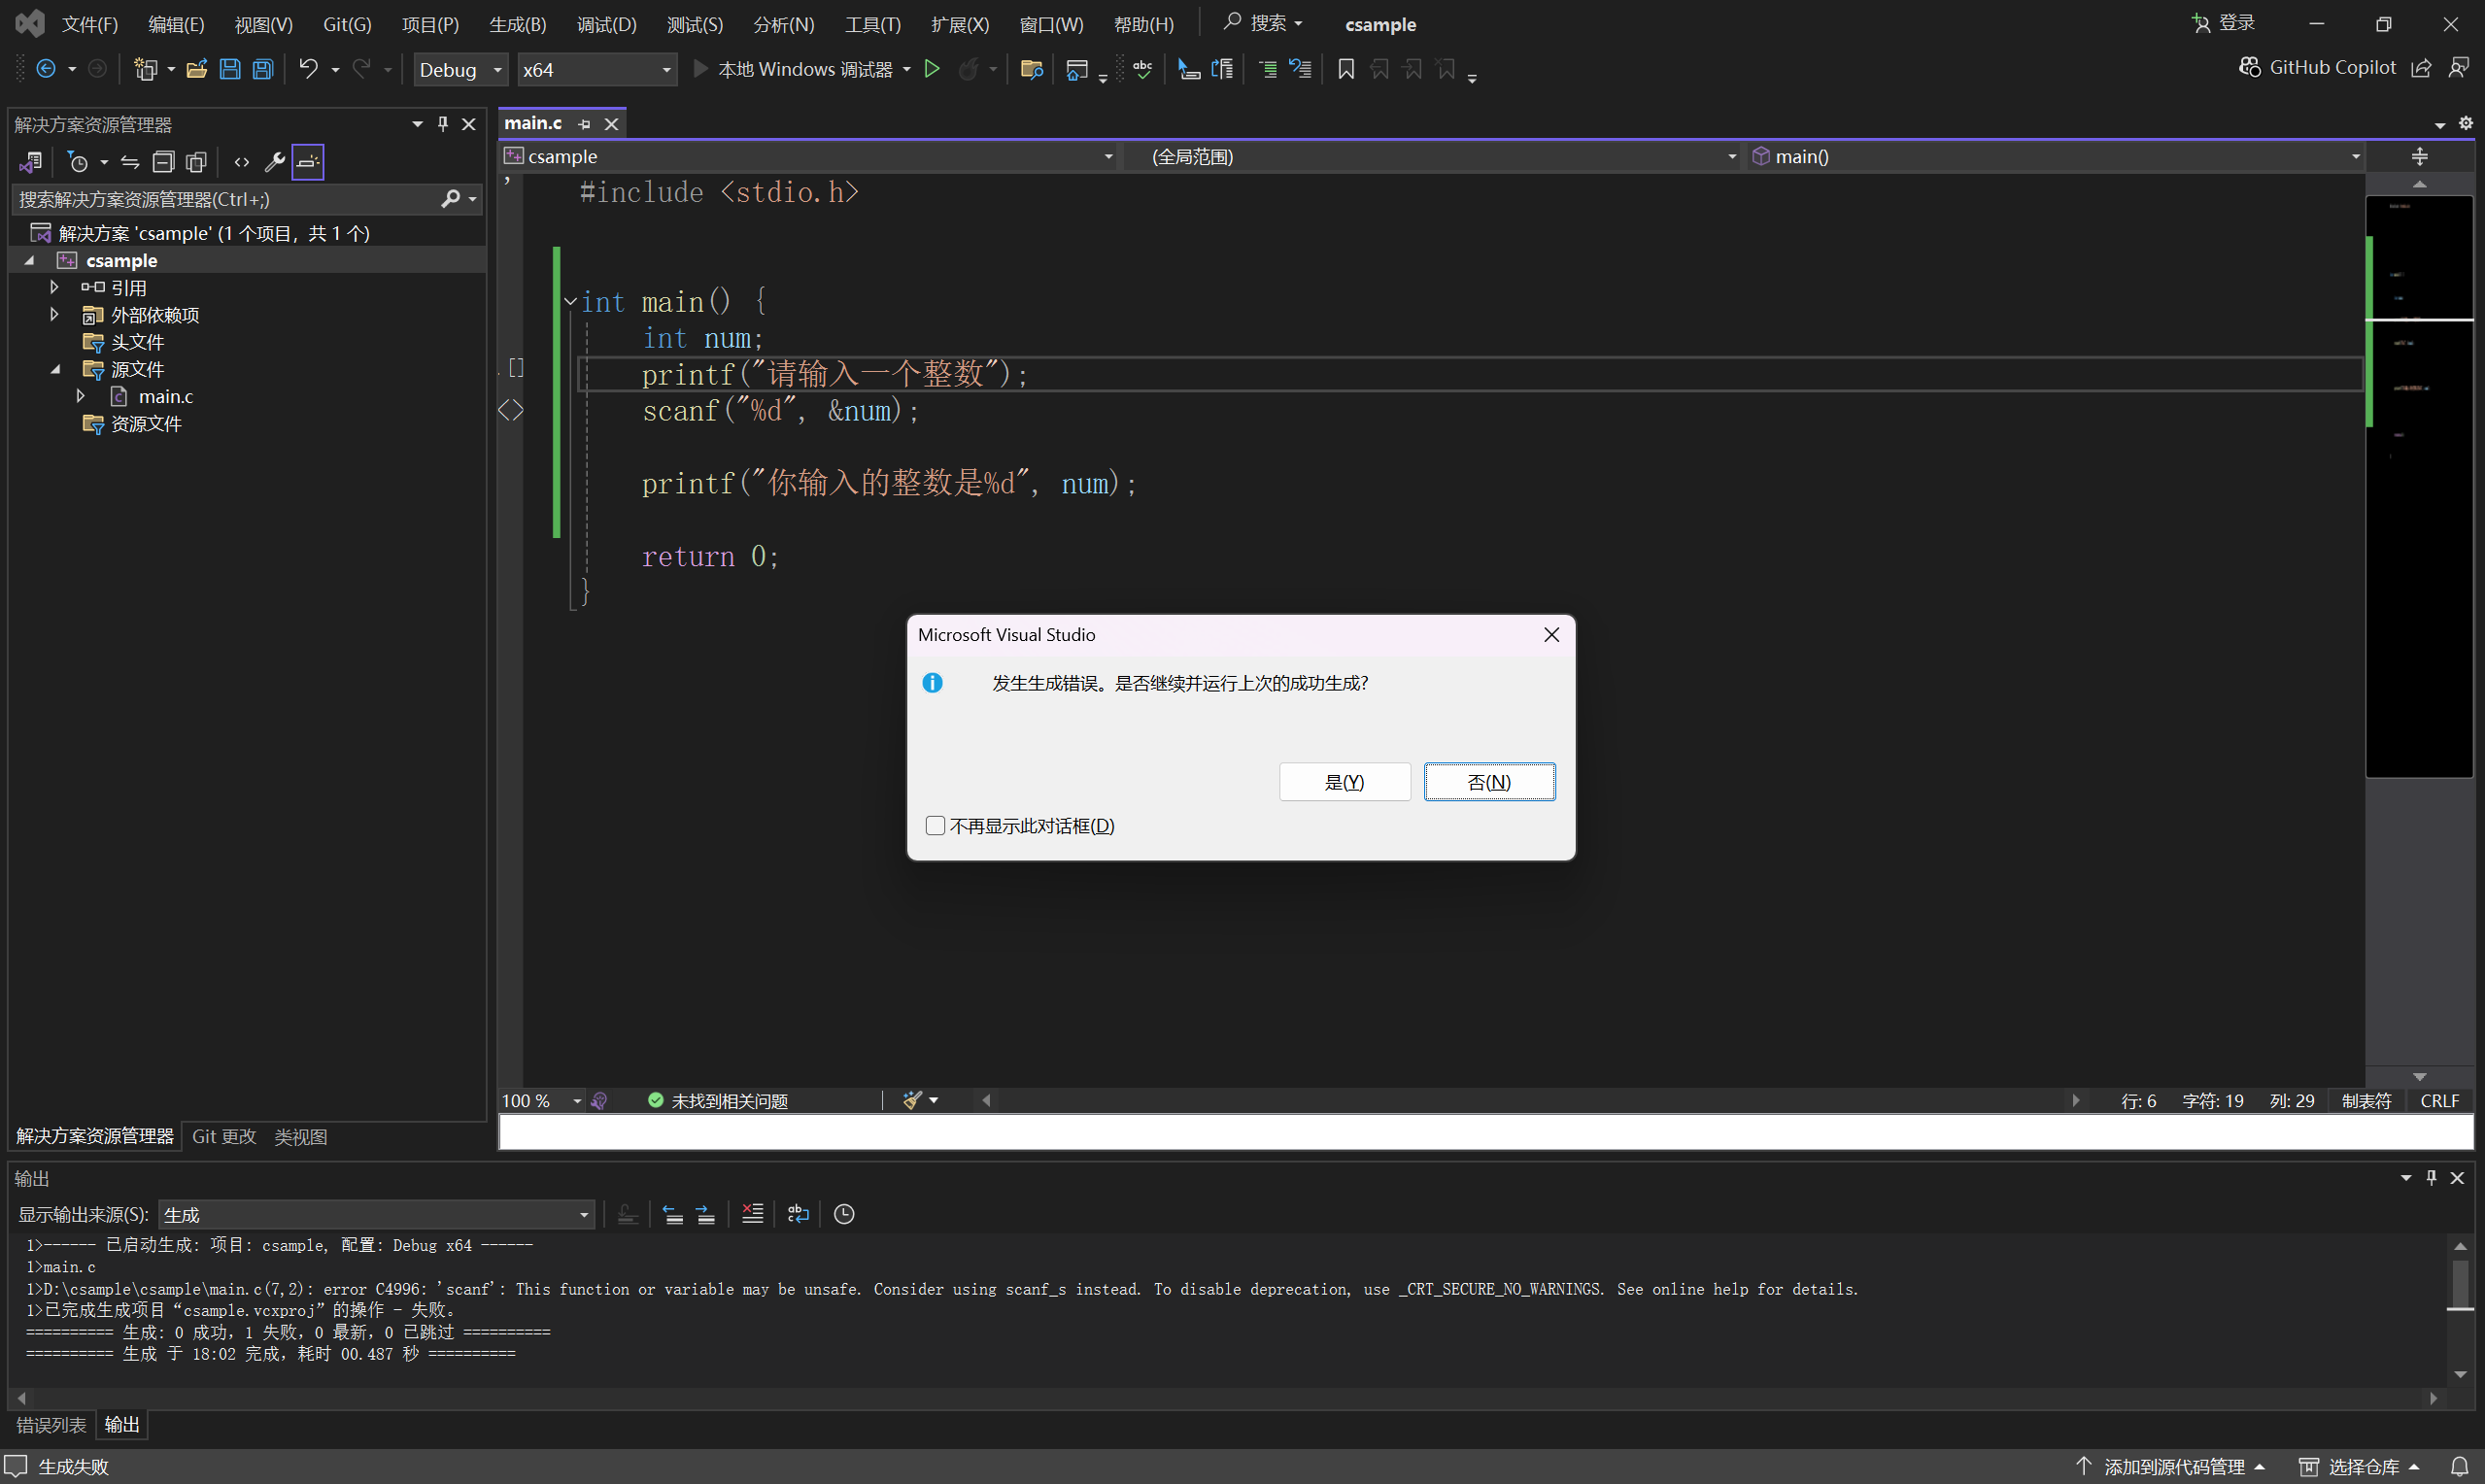
\includegraphics[width=0.8\textwidth, height=0.4\textheight]{images/1标准输入报错.png}
\end{figure}

这个窗口的意思是我们的代码有问题,过不了编译。在实际编程开发时,由于我们很难做到一次就尽善尽美,所以常常会遇到这个窗口。还好代码的试错成本是很低的,我们只需要着手去修补自己的代码即可。我们点击否,注意到visual stdio最下面出现了这样的文本

\begin{figure}[H]
    \centering
    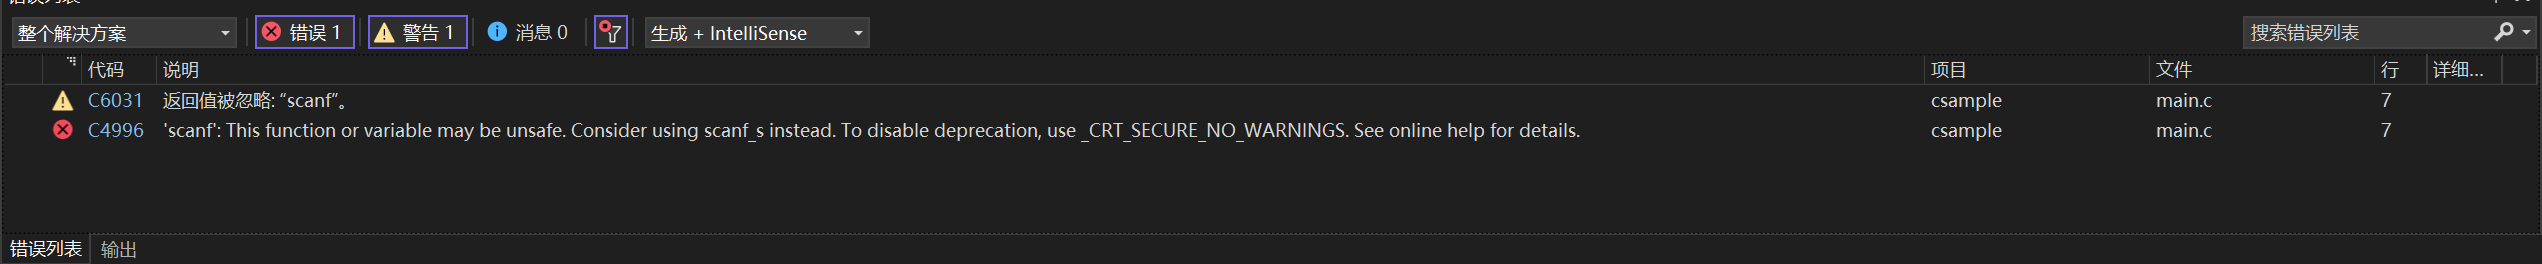
\includegraphics[width=\textwidth, height=0.2\textheight]{images/1ide错误提示.png}
\end{figure}

带有黄色警示标志的叫做警告(warning),它的意义是代码可能有一些不符合规范的地方,需要修改,但是不改也能运行。而红色标志的叫做错误(error),它的意义是这里的代码完全有问题,过不了编译,程序运行不了。我们必须要消除代码中所有的error,也要尽可能消除所有的warning。

我们开始着手消灭这个error,它的提示信息说“This function or variable may be unsafe. Consider using scanf\_s instead. To disable deprecation, use \_CRT\_SECURE\_NO\_WARNINGS. See online help for details.”

翻译成中文,就是“这个函数或者变量可能不安全。考虑使用scanf\_s替代。若要取消废弃(检查),使用\_CRT\_SECURE\_NO\_WARNINGS。详细信息见在线帮助。”。它的意思就是说,我们用的这个scanf函数不安全,已经废弃了,要么我们换用scanf\_s,要么我们加上\_CRT\_SECURE\_NO\_WARNINGS来强行使用废弃的函数。

实际上,scanf由于设计不当,会有缓冲区溢出(buffer overflow)的风险,所以我们确实不应该使用它。但是呢,只有我们使用的visual stdio会报这个错误,其它ide不会强制要求你换,而且大部分的c语言试题和c语言教程仍在使用scanf,所以我们采取强制使用废弃函数的方法来消除这个error。

在visual stdio的项目右键,点击属性,点击“C/C++”,点击“预处理器”,点击“预处理器定义”,随后点击右边出现的小箭头,点击“<编辑>”,单独一行输入“\_CRT\_SECURE\_NO\_WARNINGS”,点击“确定”即可。

此时我们再运行代码,终端首先变成这样

\begin{figure}[H]
    \centering
    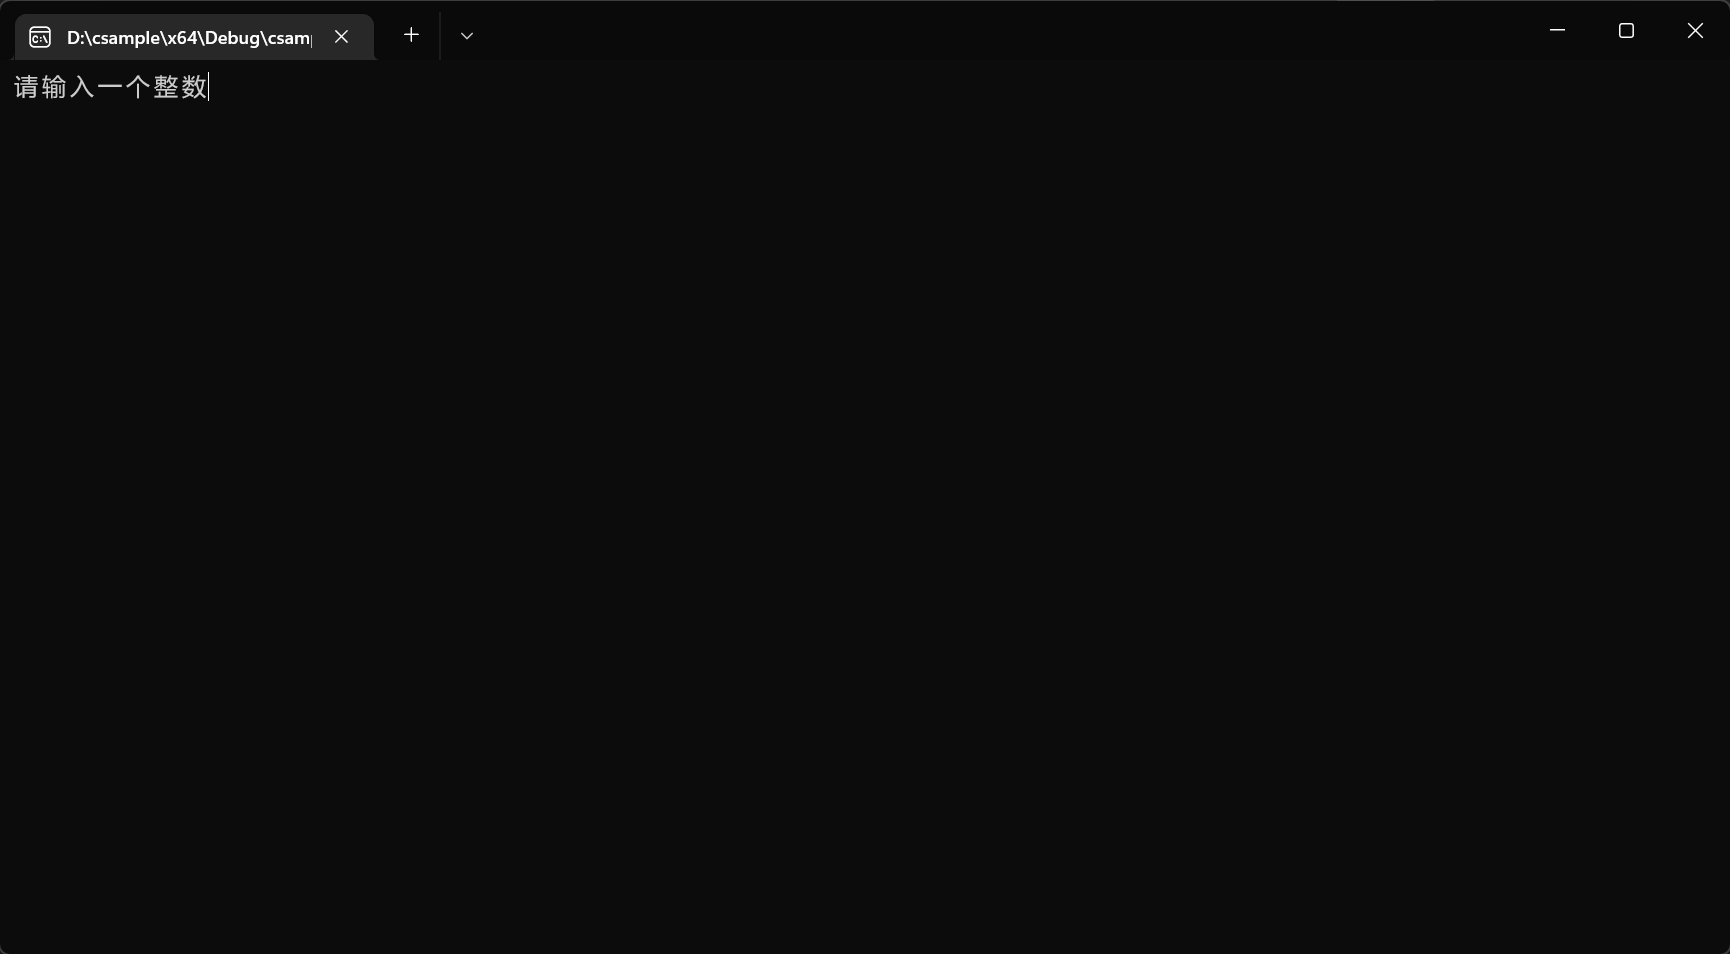
\includegraphics[width=0.8\textwidth, height=0.3\textheight]{images/1scanf首次.png}
\end{figure}

此时我们输入一个数字,点击回车,出现了这样的效果

\begin{figure}[H]
    \centering
    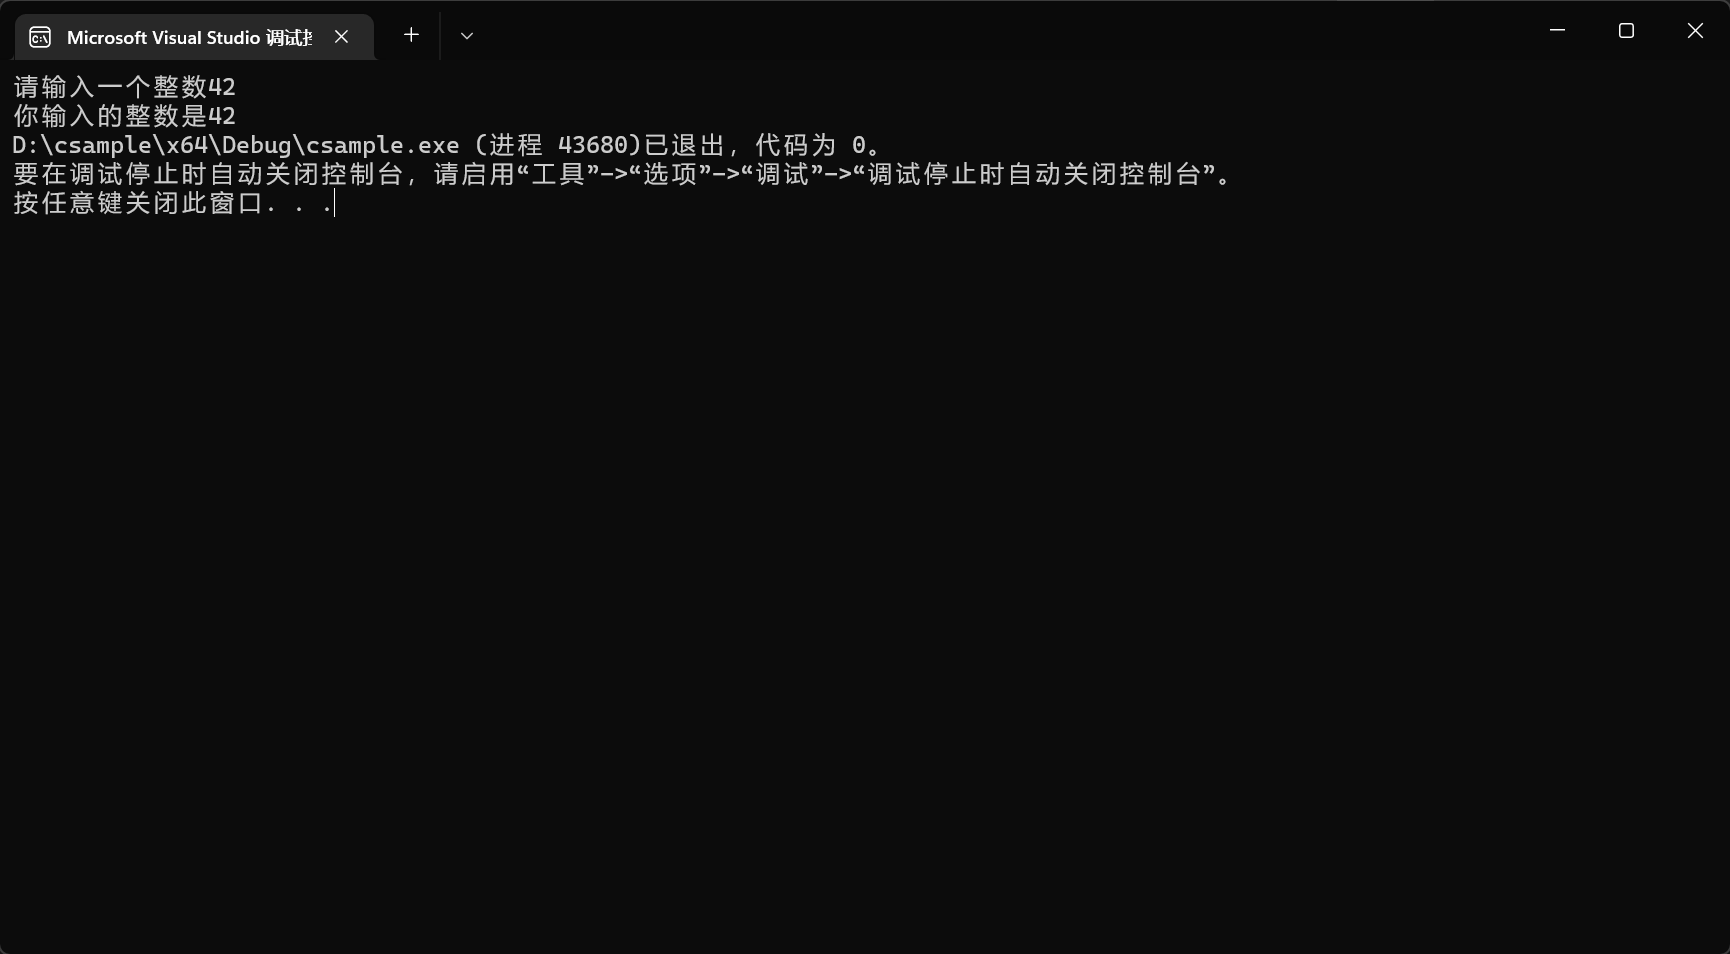
\includegraphics[width=0.8\textwidth, height=0.3\textheight]{images/1scanf完成.png}
\end{figure}

如果我们要进行的是更复杂的输入呢?比如,我们需要数学、语文和英语三科成绩,那么可以这样写

\begin{lstlisting}[language=C]
    #include <stdio.h>

    int main() {
        int math_grade;
        int chinese_grade;
        int english_grade;

        printf("请输入数学、语文、英语成绩");
        scanf("%d %d %d", &math_grade, &chinese_grade, &english_grade);

        printf("三科成绩分别是:%d, %d, %d", math_grade, chinese_grade, english_grade);
        
        return 0;
    } 
\end{lstlisting}

我们只需要按照这样输入:120 130 140,就能输出正确的成绩了。如果我们希望输入是120,130,140,那么就把scanf的一行改成

\begin{lstlisting}[language=C]
    scanf("%d,%d,%d", &math_grade, &chinese_grade, &english_grade);
\end{lstlisting}

这样我们就找到了规律,scanf的引号内的部分就像是一个模板,只有输入与模板对应,函数才正常运行。不信的话,我们可以试试在修改后的代码输入120 130 140,会得到这样的结果

\begin{figure}[H]
    \centering
    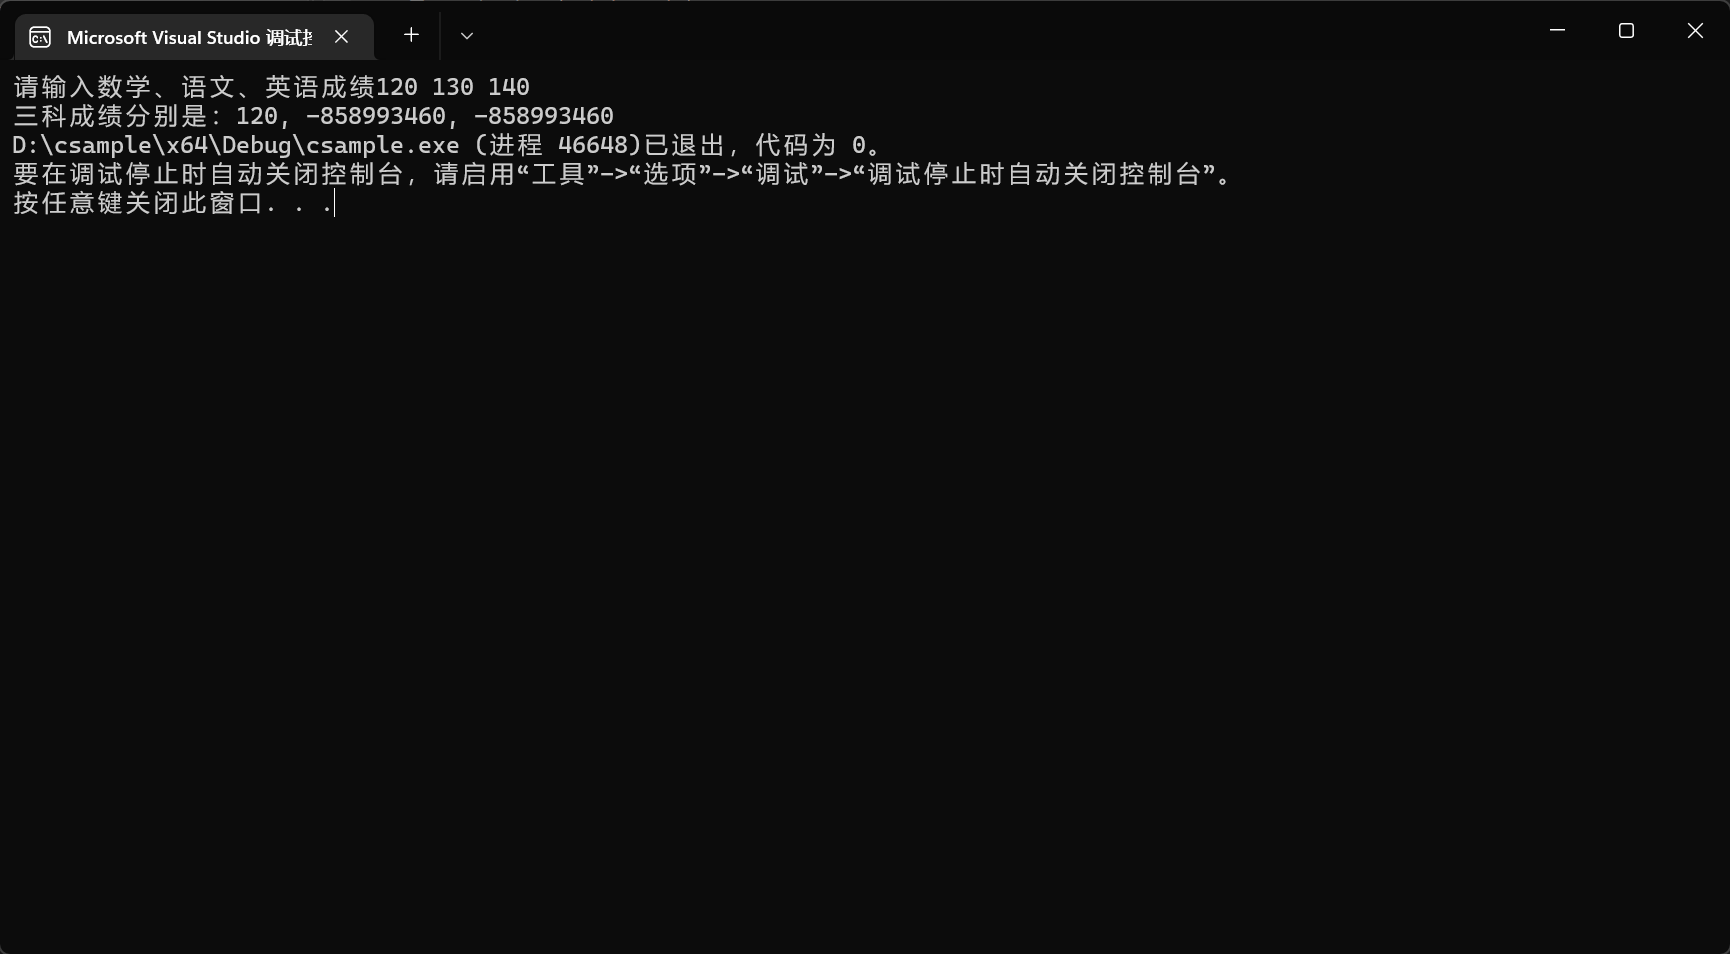
\includegraphics[width=0.8\textwidth, height=0.3\textheight]{images/1scanf出错.png}
\end{figure}

非常抽象是不是?你知道更抽象的是什么吗?假如我们使用其它编译器,那么会得到不同的结果\footnote{类似的一段代码,以120 130 140作为输入,64位电脑,处理器intel ultra9,在win11,msvc编译下运行结果为120, -858993460, -858993460;ubuntu,gcc编译下结果为120, 4096, 0;ubuntu,clang编译下结果为120, 0, 4096}。这是因为我们的输入没有符合模板的需求,模板需要我们在每两个成绩间使用英语逗号分割,我们用的却是空格,这种情况被称作未定义行为(undefined behavior),这是c语言中比较难以预测的一种的错误,我们后续会详细讲解。不知道各位记不记得,我们在解决那个error时,留了个warning尚未处理?它说我们没有使用scanf的返回值,这个“返回值”就是用来解决这个问题的,我们学习到函数时会专门提到。
